\documentclass[a4paper]{article} % you can use the same options as for article class

%%%%%%%%%%%%%%%%%%%%%%%%%%%%%%%%%%%%%% Meta Information %%%%%%%%%%%%%%%%%%%%%%%%%%%%%%%%%%%%%%

\def\muni{Masaryk University}
\def\uvt{Institute of Computer Science}
\def\street{Botanick\'{a} 68a}
\def\psc{602\,00 Brno}
\def\contactemail{husakm@ics.muni.cz}

\def\projectname{AIDA Framework}

\def\reportauthor{Martin Hus\'{a}k, Jaroslav Ka\v{s}par, Milan \v{Z}iaran}
\def\reporttitle{User Manual \& Documentation}

%%%%%%%%%%%%%%%%%%%%%%%%%%%%%%%%%%%%%% Included Packages %%%%%%%%%%%%%%%%%%%%%%%%%%%%%%%%%%%%%%

\usepackage[paper=a4paper,top=2.5cm,bottom=2.5cm,left=2.5cm,right=2.5cm,bottom=2.5cm,foot=1cm]{geometry}
\usepackage{cmap}       % cut and past support for iso-8859-2 characters
\usepackage[utf8]{inputenc}
\usepackage[default,osfigures,scale=0.5]{opensans}
\usepackage[T1]{fontenc}
\usepackage[hyphens]{url}
\usepackage{hyperref}
\usepackage{array}
\usepackage[table, usenames, dvipsnames]{xcolor}
\usepackage{indentfirst}
\usepackage{enumitem}
\usepackage{graphicx}
\DeclareGraphicsExtensions{.pdf, .ps, .eps, .png}

%%%%%%%%%%%%%%%%%%%%%%%%%%%%%%%%%%%%%% Colors %%%%%%%%%%%%%%%%%%%%%%%%%%%%%%%%%%%%%%

\definecolor{projectcolor}{RGB}{93,118,168}
\definecolor{textcolor}{RGB}{90,90,90}

%%%%%%%%%%%%%%%%%%%%%%%%%%%%%%%%%%%%%% Settings for pdf output %%%%%%%%%%%%%%%%%%%%%%%%%%%%%%%%%%%%%%

\hypersetup{%
pdftitle   = {\reporttitle},
pdfauthor  = {\reportauthor},
pdfsubject = {\projectname},
pdfkeywords= {},
%
unicode=true,                % czech in bookmarks
bookmarks=true,              % turn on creation of bookmarks
bookmarksopen=false,         % expand subsections in bookmark tab
bookmarksnumbered = true,    % chapter numbers in bookmarks
bookmarksopenlevel = 5,
%
pdfpagemode=UseOutlines,     % UseThumbs, UseOutlines (turn on bookmarks), FullScreen, None
pdfpagelayout=SinglePage,    % SinglePage, OneColumn, TwoColumnLeft, TwoColumnRight
pdfstartview=FitV,           % Fit, FitB, FitH, FitV
%
backref = false,
linkcolor = textcolor,
citecolor = textcolor,
urlcolor = textcolor,
colorlinks = true,           % on/off link boxes
hyperindex=true,
plainpages=false,            % fix duplicated pages when roman/arabic numbering is used
%
}

%%%%%%%%%%%%%%%%%%%%%%%%%%%%%%%%%%%%%% Document formating %%%%%%%%%%%%%%%%%%%%%%%%%%%%%%%%%%%%%%

\renewcommand{\sfdefault}{opensans}
\renewcommand{\familydefault}{\sfdefault}
\renewcommand{\normalsize}{\fontsize{12}{15}\selectfont\color{textcolor}}

\tolerance 9999 % big white space tolerance for better typesetting and text hyphenation

\def\verbatim@font{\color{textcolor}} % color of verbatim text

\makeatletter       % section title formating
\renewcommand\section{\@startsection {section}{1}{\z@}%
                   {-3.5ex \@plus -1ex \@minus -.2ex}%
                   {2.3ex \@plus.2ex}%
                   {\normalfont\sffamily\Large\bfseries\color{projectcolor}}}
\renewcommand\subsection{\@startsection{subsection}{2}{\z@}%
                   {-3.25ex\@plus -1ex \@minus -.2ex}%
                   {1.5ex \@plus .2ex}%
                   {\normalfont\sffamily\large\bfseries\color{projectcolor}}}
\renewcommand\subsubsection{\@startsection{subsubsection}{3}{\z@}%
                   {-3.25ex\@plus -1ex \@minus -.2ex}%
                   {1.5ex \@plus .2ex}%
                   {\normalfont\sffamily\normalsize\bfseries\color{projectcolor}}}
\makeatother

\newenvironment{itemize*}%
{\begin{itemize}%
    \setlength{\itemsep}{0pt}%
    \setlength{\parskip}{0pt}%
}{\end{itemize}}

\usepackage[pages=some,scale=1,angle=0,opacity=1]{background}
\newcommand\BackImage[2][scale=1]{%
\BgThispage
\backgroundsetup{
  contents={\includegraphics[#1]{#2}}
  }
}
\usepackage[absolute,overlay]{textpos}

% fancy verbatim and listings
\usepackage{fancyvrb}
\usepackage{listings}
\definecolor{listingbg}{RGB}{242,242,242}
\lstset{
	basicstyle=\footnotesize\ttfamily,
	inputencoding=utf8,
% 	extendedchars=true,
% 	literate={á}{\'{a}}1 {š}{\v{s}}1,
  escapeinside={\%*}{*)},
	captionpos=b,
	backgroundcolor=\color{listingbg},
	framesep=4pt,
	frame=single,
	breaklines=true,
	rulecolor=\color{listingbg},
	aboveskip=10pt,
	xleftmargin=1cm
}

\begin{document}

% do not indent first line in a paragraph
\setlength{\parindent}{0cm}

% title page
{
\BackImage[width=1.4\textwidth]{fig/titlepage_bg}
\pdfbookmark[1]{Title page}{pdf_first_page}

\vspace*{5cm}

\color{white}
  \begin{center}
  \vspace{2cm} {\Huge \projectname}

  \vspace{1cm} {\huge\bfseries\MakeUppercase{\reporttitle}}
  \end{center}

  \begin{textblock}{3}(1,10)
      \hyphenpenalty=10000 % prevent names from hyphenating
         \begin{tabular}{rl }
            Authors & \reportauthor \\
             & \\
            Contact email & \contactemail \\
             & \\
            Contact address & \muni \\
             & \uvt \\
             & \street \\
             & \psc \\
          \end{tabular}
      \hyphenpenalty=0
  \end{textblock}
  \cleardoublepage
}

\normalfont

% content page

\pdfbookmark[1]{Content}{pdf_contents}

\setcounter{tocdepth}{2}

\tableofcontents

\cleardoublepage

\section{Introduction}

AIDA is an analytical framework for processing intrusion detection alerts with a focus on alert correlation and predictive analytics. The framework contains components that filter, aggregate, and correlate the alerts, and predict future security events using the predictive rules distilled from historical records. The components are based on stream processing and use selected features of data mining (namely sequential rule mining) and complex event processing. The framework was designed to be deployed as an analytical component of an alert processing platform. Alternatively, it can be deployed locally for experimentations over datasets.

\begin{figure}[h]
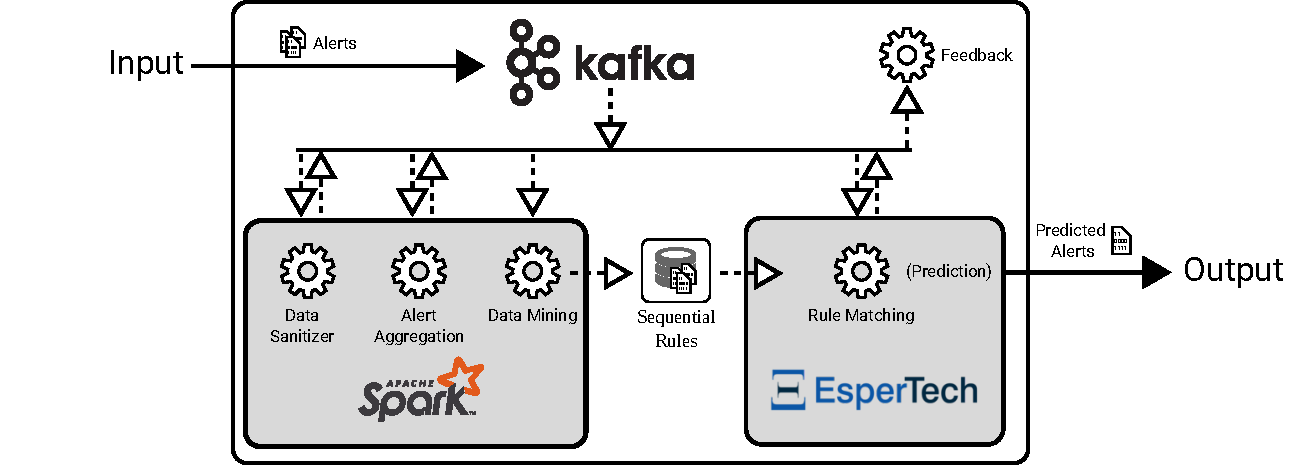
\includegraphics[width=\textwidth]{fig/aida_schema}
\caption{Example of a sequential rule.}
\label{fig:aida}
\end{figure}

Schema of the AIDA framework is presented in Figure~\ref{fig:aida}. The central component of the framework is Kafka message broker\footnote{\url{https://kafka.apache.org/}} that takes the data from inputs and distributes them among the other components while ensuring the correct order of processing of the alerts. Particular components can then be found in two component groups based on their underlying software platform. On the left side, we can see a group of components implemented as applications in Spark analytical engine\footnote{\url{https://spark.apache.org/}}. These applications typically receive a stream of alerts from Kafka, process them, and return them to Kafka. Some applications, such as the Data Mining component, have another output, such as a database for long-term storage of results of data processing. On the right side of the schema, we can see an application based on Esper\footnote{\url{http://www.espertech.com/esper/}}, another event stream processing framework. The component implemented using Esper uses its features, such as a powerful query language, for the benefits of the whole AIDA framework. The Rule Matching component is also one of the few that provide outputs outside the framework. Outputs are in the same form as inputs, i.e., intrusion detection alerts, so the output channel is implemented analogously. More details on particular components are discussed further in this document.

\bigskip

AIDA framework expects the input alerts to be formatted in IDEA (Intrusion Detection Extensible Alert) format\footnote{\url{https://idea.cesnet.cz/en/index}}. IDEA is inspired by IDMEF, a popular alert exchange format\footnote{\url{https://www.ietf.org/rfc/rfc4765.txt}}. Contrary to IDMEF, IDEA is extensible, includes a classification of alerts based on taxonomies from CSIRT communities, and is adjusted to suit practical needs. See the example of an intrusion detection alert in IDEA format in Figure~\ref{fig:idea}.

\begin{figure}[h]
\begin{lstlisting}[]
{
  "Format": "IDEA0",
  "ID":"f62537c2-77b8-49c7-a0a2-24c4b81b20f8",
  "CorrelID": [ % IDs of preceding alerts
        "3688762d-2efa-44a8-9ea5-34a57b3ae0c7",
        "ae6d9ac6-6389-407f-9d7e-58b9692c6eaa"
      ],
  "DetectTime": "2019-03-16T12:17:21.609+00:00",
  "Category": ["Attempt.Login"],
  "Confidence": "0.6111",
  "Description": "The source IP address follows a known pattern that is expected to continue with the event described in this message.",
  "Note": "OrganizationA.Honeypot1_Recon.Scanning_22, OrganizationB.IDS1_Attempt.Login_22 ==> OrganizationA.IDS1_Attempt.Login_22",
  "Source": [{"IP4": ["10.11.12.13"]}],
  "Target": [{"Port":[22]}],
  "Node": [
    { % Node referencing the AIDA Framework
      "Name": "OrganizationX.AIDA",
      "SW": "AIDA",
      "Type": ["Correlation", "Statistical"]
    },
    { % Node derived from the rule
      "Name": "OrganizationA.IDS1"
    }
  ]
}
\end{lstlisting}
\caption{Example of an intrusion detection alert in IDEA format.}
\label{fig:idea}
\end{figure}

AIDA framework extracts sequential rules from the intrusion detection alerts. The sequential rules are then used to predict upcoming attacks. An example of a sequential rule is presented in Figure~\ref{fig:seqrule}. It consists of ordered $n$-tuples (sensor name, type of event, destination port) and support and confidence values. The $n$-tuples fold two groups; the first group implies the second group. Support value indicates the number of sequences in the sequential database that conform to the rule divided by the total number of all the sequences. The confidence value is a conditional probability of the second part of the rule given the first part of the rule.

\begin{figure}[h]
\begin{lstlisting}[]
OrganizationA.Honeypot1_Recon.Scanning_22,
OrganizationB.IDS1_Attempt.Login_22
==>
OrganizationA.IDS1_Attempt.Login_22
#SUPP: 0.0011 #CONF: 0.6111
\end{lstlisting}
\caption{Example of a sequential rule.}
\label{fig:seqrule}
\end{figure}

The remainder of this documents contains a user guide, installation instructions, and technical documentation. See the user guide for a quick start on how to work with AIDA framework, either via command line or via graphical interface. The quick start should be sufficient to those users, who wish to run AIDA framework locally, e.g., to experiment over datasets. Installation instructions are recommended for users who want to deploy AIDA framework in their environment, and run it operationally. Finally, the technical documentation is intended for developers and advanced users interested in the implementation and exact procedures executed by the framework.

\cleardoublepage

\section{User Guide}

The user has two options on how to use the AIDA framework. In he first part of the user guide, we provide a quick start using a command line that provides full control over the data and their processing. The second part of user guide describes quick start using web interface (dashboard) that is recommended for users that need only basic functionality or prefer data visualizations.

\subsection{Quick Start Using Command Line}

For a quick start using command line, go to the provision directory and run Vagrant:

\begin{lstlisting}[]
cd provision
vagrant up
\end{lstlisting}

AIDA framework will start in few minutes. Then, send your data to the framework using the following command (you need to have netcat installed):

\begin{lstlisting}[]
nc localhost 4164 < path_to_file_with_your_data
\end{lstlisting}

If you do not have your own data, we recommend trying AIDA framework out with our dataset\footnote{\url{http://dx.doi.org/10.17632/p6tym3fghz.1}}. Download and unzip the main file in the datase (dataset.idea.zip) and use it in the command above.

% TODO vagrant ssh

\subsubsection*{Run data mining}

Trigger the data mining procedure (otherwise, it starts every 24 hours that you would have to wait):

\begin{lstlisting}[]
sudo systemctl start mining
\end{lstlisting}

Check the logs of the data mining component:

\begin{lstlisting}[]
sudo journalctl -u mining
\end{lstlisting}

\subsubsection*{Update rules}

Open the database with the mined rules:

\begin{lstlisting}[]
sqlite3 /var/aida/rules/rule.db
\end{lstlisting}

Check the rules in the database:

\begin{lstlisting}[]
select * from rule;
\end{lstlisting}

Activate all the rules so that they are used by the rule matching component:

\begin{lstlisting}[]
update rule set active=1;
\end{lstlisting}

Restart matching component to start matching activated rules:

\begin{lstlisting}[]
sudo systemctl restart matching
\end{lstlisting}

Send some more data into AIDA, they will be matched against the rules to predict upcoming events:

\begin{lstlisting}[]
nc localhost 4164 < path_to_file_with_your_data
\end{lstlisting}

\subsubsection*{Check outputs}

Predicted rules are saved in the root directory of this repository in `predictions.json` file.

You can also get the predictions directly from Kafka:

\begin{lstlisting}[]
`/opt/kafka/bin/kafka-console-consumer.sh --bootstrap-server localhost:9092 --topic predictions --from-beginning`
\end{lstlisting}

\cleardoublepage

\subsection{Quick Start Using AIDA Dashboard}

For a quick start using AIDA dashboard, go to the provision directory and run Vagrant:

\begin{lstlisting}[]
cd provision
vagrant up
\end{lstlisting}

AIDA framework will start in few minutes. When everything is up and running, open the dashboard on the following URL:

\begin{lstlisting}[]
http://localhost:8080/
\end{lstlisting}

You should see the login page. Type in the following default credentials:
\begin{itemize}[noitemsep,nolistsep]
  \item[] Username: admin
  \item[] Password: aida.admin
\end{itemize}
The login page looks as follows:

\begin{figure}[h]
  \centering
  
\includegraphics[width=0.75\textwidth]{fig/dashboard_login}
\end{figure}

After the login, you should the Overview panel with the status of the components of the system. Green circles indicate running component, red indicated problems with the component. Hover cursor over the icon of the component, a hover text with status text and last lines in log of the component will appear. If you see black circles, there are no information on status available. In such case, check the system.

\begin{figure}[h]
  \centering
  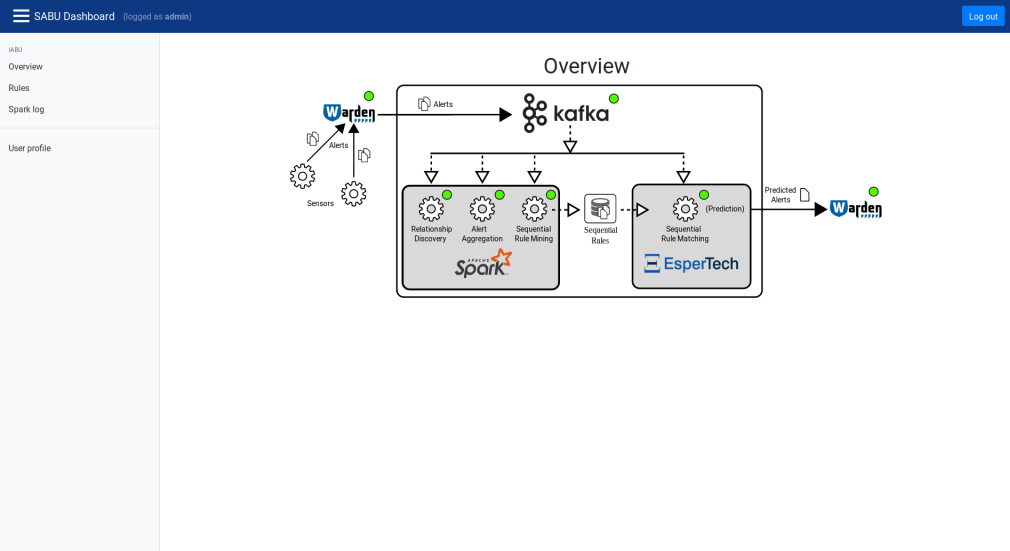
\includegraphics[width=0.75\textwidth]{fig/dashboard_overview}
\end{figure}

On the left side of the screen, you can see a navigation panel with links to other tabs. The \textbf{Rules} tab allows the user to go through the mined rules in and activate or inactivate them. The first table from top of the poge shows the rules mined on a given day. Default is the current day, user may change the day usign the calender in the right top corner. The second table shows all the active rules. Both tables show read or green circles that indicate if the rule is active or not. Click them to change the status and activate or inactivate the rule on the line. Finally, at the bottom of the page, there is a box where users may enter their own rules. Fill all the fields and click \textbf{Submit} to add your custom rule to the database.

\begin{figure}[h]
  \centering
  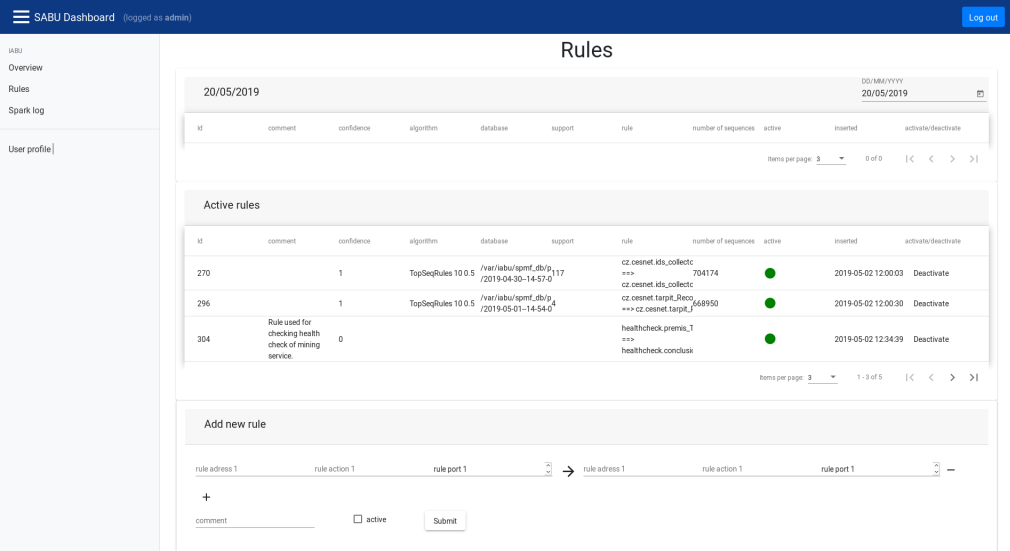
\includegraphics[width=0.75\textwidth]{fig/dashboard_rules}
\end{figure}

Users interested in performance of the framework should see the panel \textbf{Spark log}, where they can access the user interface of Spark framework, on which many components are based. Information on the number and load of workers, memory consumptions, and time to finish jobs are presented there.

\begin{figure}[h]
  \centering
  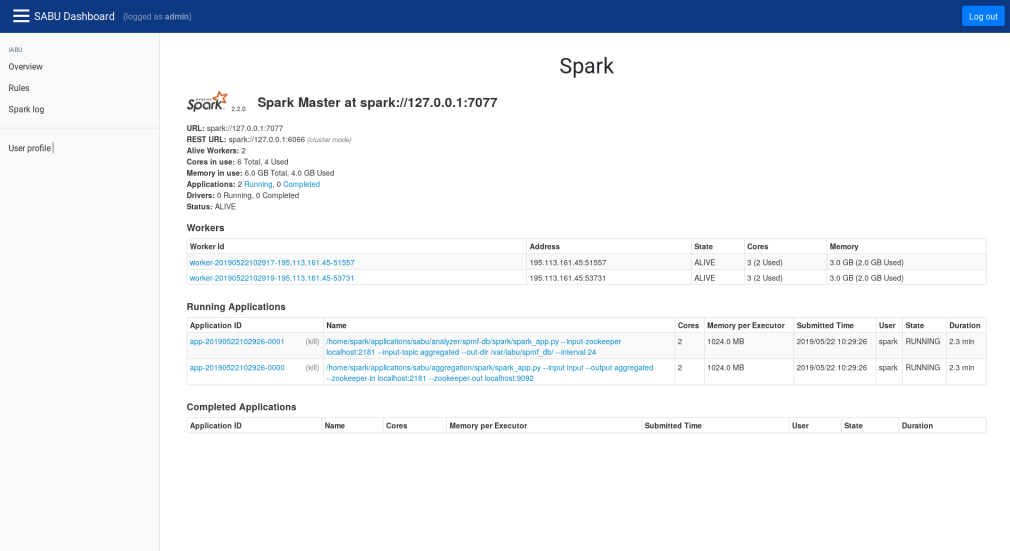
\includegraphics[width=0.75\textwidth]{fig/dashboard_spark}
\end{figure}

Finally, for the configuration of the dashboard, visit the following URL:

\begin{lstlisting}[]
http://localhost:8000/admin/
\end{lstlisting}

to access the configuration page. Use the same credentials as for the dashboard, the defaults are:
\begin{itemize}[noitemsep,nolistsep]
  \item[] Username: admin
  \item[] Password: aida.admin
\end{itemize}
In the configuration, you can add or remove user accounts, and customize the framework.

\cleardoublepage

\section{Installation Instructions}

Simplest way how to install and use AIDA is by running vagrant box \texttt{vagrant up} from \texttt{provision} directory. If you want to install AIDA on an already existing machine, you can follow the following instructions. There is a Quick Installation section whereby you can install AIDA just by running Ansible playbook. Alternatively, you can install AIDA manually step by step from the instructions in Manual Installation section.

\subsection{Prerequisites}

Installed Ubuntu 18.04.2 and AIDA repository downloaded or cloned into \texttt{/vagrant} directory. You can choose any other directory, but we will refer the repository root as \texttt{/vagrant}. You should have also installed the following dependencies:
\begin{itemize}[nolistsep,noitemsep]
    \item Installed Java JDK version 1.8
    \item Installed Maven version 3.6
    \item Installed Python 2.7 as \texttt{python}
    \item Installed Python 3.6 as \texttt{python3}
    \item Installed Pip for python 2.7 as \texttt{pip}
    \item Installed Pip for python 3.6 as \texttt{pip3}
\end{itemize}
You can install the above prerequisites by running:
\begin{lstlisting}
$ sudo apt-get update
$ sudo apt-get -y install openjdk-8-jdk maven python-pip python3-pip
$ sudo update-java-alternatives --set java-1.8.0-openjdk-amd64
\end{lstlisting}

\subsection{Quick Installation}

The simplest way how to install AIDA is by running Ansible playbook.

You have to have Ansible installed. You can do it by running following command:

\begin{lstlisting}
$ sudo apt-get -y install ansible
\end{lstlisting}

Then run ansible playbook:

\begin{lstlisting}
$ cd /vagrant/provision/ansible
$ ansible-playbook -i inventory-local.ini install-aida.yml
\end{lstlisting}

Note that the Ansible will also install Java 8, Python 3 and other packages listed in prerequisites section.

You can check that the main AIDA services are up and running by running.
\begin{lstlisting}
$ sudo systemctl status aida-input sanitization aggregation matching
\end{lstlisting}

% Install Dashboard
% TODO

\subsection{Manual Installation}

This section provides step-by-step instructions on how to install AIDA framework on an existing machine without using Ansible. This process is more complicated and, thus, is recommended only to advanced users, and users interesting in implementation of the framework. During the installation, we are going to create dedicated user accounts for almost every AIDA service. However, you can create just one user for all the AIDA services, and run the framework under one user.

\subsubsection{Install Kafka}

We will install Kafka and Zookeper and run single Kafka broker on the machine.

First, create Kafka user:
\begin{lstlisting}
$ sudo useradd -M kafka
\end{lstlisting}

Install Zookeper service:
\begin{lstlisting}
$ sudo apt-get -y install zookeeperd
\end{lstlisting}

Download Kafka binary into \texttt{/opt/kafka}:
\begin{lstlisting}
$ sudo su
# mkdir /opt/kafka
# cd /opt/kafka
# wget https://archive.apache.org/dist/kafka/2.3.0/kafka_2.12-2.3.0.tgz -O kafka.tgz
# tar -xzf kafka.tgz --strip-components=1
# rm kafka.tgz
# chown -R kafka:kafka ./
\end{lstlisting}

Create systemd unit file for \texttt{kafka} service:
\begin{lstlisting}
$ sudo cp /vagrant/provision/ansible/roles/kafka/templates/kafka.service.j2 /etc/systemd/system/kafka.service
\end{lstlisting}

Then you have to replace following placeholders in the newly created file \texttt{/etc/systemd/system/kafka.service} as follows:
\begin{itemize}[noitemsep,nolistsep]
\item \texttt{\{\{ kafka\_user \}\}} with \texttt{kafka} or other user you had chosen to use
\item \texttt{\{\{ kafka\_dir \}\}} with \texttt{/opt/kafka}
\end{itemize}

Create systemd unit file for \texttt{kafka-topic} services:
\begin{lstlisting}
$ sudo cp /vagrant/provision/ansible/roles/kafka/templates/kafka-topic.service.j2 /etc/systemd/system/kafka-topic@.service
\end{lstlisting}
Then, replace the same placeholders as in previous step in the newly created file.

Now you can start the \texttt{kafka} service by running:
\begin{lstlisting}
$ sudo systemctl start kafka
\end{lstlisting}

And check that it's running:
\begin{lstlisting}
$ sudo systemctl status kafka
\end{lstlisting}

Also check that \texttt{kafka-topic} service is working by creating \texttt{input} topic:
\begin{lstlisting}
$ sudo systemctl start kafka-topic@input
$ sudo systemctl status kafka-topic@input
\end{lstlisting}


\subsubsection{Install Spark}

We will install and configure Spark so we are able to run Spark applications in local mode.

First, create Spark user:
\begin{lstlisting}
$ sudo useradd -M spark
\end{lstlisting}

Download Spark binary to the \textt{/opt/spark/spark} directory:
\begin{lstlisting}
$ sudo su
# mkdir -p /opt/spark/spark
# cd /opt/spark/spark
# wget https://archive.apache.org/dist/spark/spark-2.4.3/spark-2.4.3-bin-hadoop2.7.tgz -O spark.tgz
# tar -xzf spark.tgz --strip-components=1
# rm spark.tgz
# wget https://search.maven.org/classic/remotecontent?filepath=org/apache/spark/spark-streaming-kafka-0-8-assembly_2.11/2.4.3/spark-streaming-kafka-0-8-assembly_2.11-2.4.3.jar -O /opt/spark/spark/jars/spark-streaming-kafka-0-8-assembly_2.11-2.4.3.jar
\end{lstlisting}

Prepare modules for Spark applications:
\begin{lstlisting}
$ sudo su
# mkdir -p /opt/spark/applications
# cp -r /vagrant/commons/commons-python /opt/spark/applications/modules
# pip3 install -r /opt/spark/applications/modules/requirements.txt
# apt-get -y install zip
# zip -j -r /opt/spark/applications{.zip,}
\end{lstlisting}

Prepare script for running Spark applications:
\begin{lstlisting}
$ sudo su
# cp /vagrant/provision/ansible/roles/spark/templates/run-application.sh.j2 /opt/spark/applications/run-application.sh
# chmod +x /opt/spark/applications/run-application.sh
\end{lstlisting}

Now, you have to replace placeholder \texttt{\{\{ spark\_home\_dir \}\}} with \texttt{/opt/spark/spark} in the \texttt{run-application.sh} file.

Create configuration file:
\begin{lstlisting}
$ sudo cp /vagrant/provision/ansible/roles/spark/templates/spark-defaults.conf.j2 /opt/spark/spark/conf/spark-defaults.conf
\end{lstlisting}

Replace placeholder \texttt{\{\{ spark\_modules\_zip \}\}} with \texttt{/opt/spark/applications/\\modules/modules.zip} in the newly created configuration file. You can also increase the \texttt{spark.driver.memory} due to available memory to be able to pass more data into AIDA.

Make \texttt{spark} user owner of the \texttt{/opt/spark} directory:
\begin{lstlisting}
$ sudo chown -R spark:spark /opt/spark/
\end{lstlisting}


\subsubsection{Install Java commons for AIDA components}

Install Java commons modules for AIDA components:
%TODO sudo or not sudo
\begin{lstlisting}
$ cd /vagrant/commons/commons-idea
$ mvn clean install
$ cd /vagrant/commons/commons-mining
$ mvn clean install
\end{lstlisting}


\subsubsection{Install aida-input service}

Install \texttt{aida-input} service which will listen on port 4164 and will send all the incoming events into AIDA:
\begin{lstlisting}
$ sudo cp /vagrant/provision/ansible/roles/aida-input/templates/aida-input.service.j2 /etc/systemd/system/aida-input.service
\end{lstlisting}

Replace following placeholders in the newly created file \texttt{/etc/systemd/system/\\aida-input.service} as follows:
\begin{itemize}[noitemsep,nolistsep]
\item \texttt{\{\{ kafka\_user \}\}} with \texttt{kafka} or other user you had chosen to use while installing Kafka
\item \texttt{\{\{ kafka\_dir \}\}} with \texttt{/opt/kafka}
\item \texttt{\{\{ aida\_input\_port \}\}} with \texttt{4164}
\end{itemize}

Run the \texttt{aida-input} service:
\begin{lstlisting}
$ sudo systemctl start aida-input
\end{lstlisting}

Check that the service is running:
\begin{lstlisting}
$ sudo systemctl status aida-input
\end{lstlisting}


\subsubsection{Install Sanitization component}

Create sanitization user:
\begin{lstlisting}
$ sudo useradd -M sanitization
\end{lstlisting}

Install sanitization:
\begin{lstlisting}
$ sudo mkdir /opt/sanitization
$ cd /vagrant/services/sanitization
$ mvn clean package
$ cp ./target/*jar-with-dependencies.jar /opt/sanitization/sanitization.jar
$ sudo chown -R sanitization:sanitization /opt/sanitization
\end{lstlisting}

Create systemd unit file for \texttt{sanitization} service:
\begin{lstlisting}
$ sudo cp /vagrant/provision/ansible/roles/sanitization/templates/sanitization.service.j2 /etc/systemd/system/sanitization.service
\end{lstlisting}

Then, replace the following placeholders in the newly created file:
\begin{itemize}[noitemsep,nolistsep]
\item \texttt{\{\{ sanitization\_user \}\}} with \texttt{sanitization} or other user you had chosen
\item \texttt{\{\{ sanitization\_dir \}\}} with \texttt{/opt/sanitization}
\end{itemize}

Run the \texttt{sanitization} service:
\begin{lstlisting}
$ sudo systemctl start sanitization
\end{lstlisting}

Check that the service is running:
\begin{lstlisting}
$ sudo systemctl status sanitization
\end{lstlisting}


\subsubsection{Install Aggregation component}

Put Aggregation Spark application into the required directory:
\begin{lstlisting}
$ sudo cp -r /vagrant/services/aggregation /opt/spark/applications/aggregation
$ sudo chown -R spark:spark /opt/spark/applications/aggregation
\end{lstlisting}

Install python dependencies:
\begin{lstlisting}
$ sudo pip3 install -r /opt/spark/applications/aggregation/requirements.txt
\end{lstlisting}

Create systemd unit file for \texttt{aggregation} service:
\begin{lstlisting}
$ sudo cp /vagrant/provision/ansible/roles/aggregation/templates/aggregation.service.j2 /etc/systemd/system/aggregation.service
\end{lstlisting}

Then replace following placeholders in newly created file:
\begin{itemize}[noitemsep,nolistsep]
\item \texttt{\{\{ spark\_user \}\}} with \texttt{spark}
\item \texttt{\{\{ spark\_run\_app\_script \}\}} with \texttt{/opt/spark/applications/run-application.sh}
\item \texttt{\{\{ aggregation\_install\_dir \}\}} with \texttt{/opt/spark/applications/aggregation}
\end{itemize}

Run the \texttt{aggregation} service:
\begin{lstlisting}
$ sudo systemctl start aggregation
\end{lstlisting}

Check that the service is running:
\begin{lstlisting}
$ sudo systemctl status aggregation
\end{lstlisting}


\subsubsection{Prepare Rules database}

We are going to create SQLite3 database file with \texttt{rule} table for mined rules.

First, create the directory:
\begin{lstlisting}
$ sudo mkdir -p /var/aida/rules
\end{lstlisting}

Install SQLite3 and create database file with required permissions:
\begin{lstlisting}
$ sudo apt-get -y install sqlite3
$ sudo sqlite3 /var/aida/rules/rule.db 'CREATE TABLE rule (id INTEGER PRIMARY KEY, inserted DATETIME DEFAULT CURRENT_TIMESTAMP, rule TEXT NOT NULL, support INTEGER, number_of_sequences INTEGER, confidence REAL, active INTEGER DEFAULT 0, comment TEXT, database TEXT, algorithm TEXT )'
$ sudo chmod 0666 /var/aida/rules/rule.db
\end{lstlisting}

\subsubsection{Install mining service}

Create mining user:
\begin{lstlisting}
$ sudo useradd -M mining
\end{lstlisting}

Install mining binary:
\begin{lstlisting}
$ sudo mkdir /opt/mining
$ cd /vagrant/services/mining
$ mvn clean
$ mvn package
$ sudo cp ./target/*jar-with-dependencies.jar /opt/mining/mining.jar
$ sudo chown mining:mining /opt/mining
\end{lstlisting}

Create systemd unit file for \texttt{mining} service:
\begin{lstlisting}
$ sudo cp /vagrant/provision/ansible/roles/mining/templates/mining.service.j2 /etc/systemd/system/mining.service
\end{lstlisting}

Then replace following placeholders in newly created unit file:
\begin{itemize}[noitemsep,nolistsep]
\item \texttt{\{\{ mining\_user \}\}} with \texttt{mining} or other user you had chosen
\item \texttt{\{\{ mining\_dir \}\}} with \texttt{/opt/mining}
\item \texttt{\{\{ database\_path \}\}} with \texttt{/var/aida/rules/rule.db}
\end{itemize}

Create systemd timer for \texttt{mining} service:
\begin{lstlisting}
$ sudo cp /vagrant/provision/ansible/roles/mining/templates/mining.timer.j2 /etc/systemd/system/mining.timer
\end{lstlisting}

Note that mining is a one-shot service. It will run the mining on all event currently available in Kafka and then finish. You can trigger the mining by starting the service:
\begin{lstlisting}
$ sudo systemctl start mining
\end{lstlisting}

Then, check it did exit successfully:
\begin{lstlisting}
$ sudo systemctl status mining
\end{lstlisting}

Alternatively, you can check the logs:
\begin{lstlisting}
$ sudo journalctl -u mining
\end{lstlisting}


\subsubsection{Install Rule Matching component}

Rule Matching component reads the rule database and predicts the upcoming alerts via matching the rules in the stream of data.

Create user for the Matching component:
\begin{lstlisting}
$ sudo useradd -M matching
\end{lstlisting}

Install binary for the Matching component:
\begin{lstlisting}
$ sudo mkdir /opt/matching
$ cd /vagrant/services/matching
$ mvn clean package
$ sudo cp ./target/*jar-with-dependencies.jar /opt/matching/matching.jar
$ sudo chown -R matching:matching /opt/matching
\end{lstlisting}

Create systemd unit file for \texttt{matching} service:
\begin{lstlisting}
$ sudo cp /vagrant/provision/ansible/roles/matching/templates/matching.service.j2 /etc/systemd/system/matching.service
\end{lstlisting}

Then replace following placeholders in newly created file:
\begin{itemize}[noitemsep,nolistsep]
\item \texttt{\{\{ matching\_user \}\}} with \texttt{matching} or other user you had chosen
\item \texttt{\{\{ matching\_dir \}\}} with \texttt{/opt/matching}
\item \texttt{\{\{ database\_path \}\}} with \texttt{/var/aida/rules/rule.db}
\end{itemize}

Run the \texttt{matching} service:
\begin{lstlisting}
$ sudo systemctl start matching
\end{lstlisting}

Check that the service is running:
\begin{lstlisting}
$ sudo systemctl status matching
\end{lstlisting}


\subsubsection{Install aida-output service}

The \texttt{aida-output} service will read predictions from Kafka and save them into file.

First, create predictions file with permission of same user used for Kafka:
\begin{lstlisting}
$ touch /vagrant/predictions.json
$ chown kafka:kafka /vagrant/predictions.json
\end{lstlisting}

Create systemd unit file for \texttt{aida-output} service:
\begin{lstlisting}
$ sudo cp /vagrant/provision/ansible/roles/aida-output/templates/aida-output.service.j2 /etc/systemd/system/aida-output.service
\end{lstlisting}

Replace following placeholders in the newly created unit file:
\begin{itemize}[noitemsep,nolistsep]
\item \texttt{\{\{ kafka\_user \}\}} with \texttt{kafka} or other user you had chosen to use while installing Kafka
\item \texttt{\{\{ kafka\_dir \}\}} with \texttt{/opt/kafka}
\item \texttt{\{\{ predictions\_file\_path \}\}} with \texttt{/vagrant/predictions.json}
\end{itemize}

Run the \texttt{aida-output} service:
\begin{lstlisting}
$ sudo systemctl start aida-output
\end{lstlisting}

Check that the service is running:
\begin{lstlisting}
$ sudo systemctl status aida-output
\end{lstlisting}


\subsubsection{Install REST API}

REST API is used for communications with the AIDA Dashboard. The API is open on port 7777. This service is not mandatory, if you are not planning to use Dashboard you can skip this part.

REST API is implemented as a Django application which will run on Apache2 with WSGI. First, install Apache2 with WSGI support for Python 3:
\begin{lstlisting}
$ sudo apt-get -y install apache2 libapache2-mod-wsgi-py3
\end{lstlisting}

REST API is getting information about the AIDA services via dbus systemd interface, so we will have to install dbus dependencies:
\begin{lstlisting}
$ sudo apt-get -y install dbus libdbus-glib-1-dev libdbus-1-dev python-dbus
\end{lstlisting}

Now, place the Django application into correct directory:
\begin{lstlisting}
$ sudo cp -r /vagrant/services/restapi  /var/www/restapi
\end{lstlisting}

Create python virtual environment for REST API:
\begin{lstlisting}
$ sudo su
# apt-get -y install python3-venv
# cd /var/www/restapi
# sudo python3 -m venv venv --system-site-packages
# source venv/bin/activate
# pip install -r requirements.txt
# deactivate
\end{lstlisting}

Create config file for the application:
\begin{lstlisting}
$ sudo mkdir /etc/aida/
$ sudo cp /vagrant/provision/ansible/roles/restapi/templates/rest.ini.j2 /etc/aida/rest.ini
\end{lstlisting}
and replace the placeholder \texttt{\{\{ database\_path \}\}} in the file with \texttt{/var/aida/rules/\\rule.db}.

Now, create the config file for Apache:
\begin{lstlisting}
$ sudo cp /vagrant/provision/ansible/roles/restapi/templates/apache2.conf.j2 /etc/apache2/sites-enabled/rest-aida.conf
\end{lstlisting}
Replace placeholders in newly created config file
\begin{itemize}[noitemsep,nolistsep]
\item \texttt{\{\{ restapi\_dir \}\}} with \texttt{/var/www/restapi}
\item \texttt{\{\{ restapiaida\_dir \}\}} with \texttt{/var/www/restapi/restapiaida}
\item \texttt{\{\{ venv\_dir \}\}} with \texttt{/var/www/restapi/venv}
\end{itemize}

Finally, restart Apache2:
\begin{lstlisting}
$ sudo systemctl restart apache2
\end{lstlisting}
and check that REST API is responding on address \texttt{localhost:7777}. For example, the following command:
\begin{lstlisting}
$ curl http://localhost:7777/componentsinfo
\end{lstlisting}
should return a JSON with status of the AIDA components.

% \subsubsection{Install Dashboard}
% 
% TODO

\cleardoublepage

\section{Technical Documentation}

This section contains the technical documentation for the AIDA framework. The documentation is provided separately for each component, starting with the description of the inputs and outputs.

\subsection{Inputs and Outputs}

Simplest way for the alerts to enter AIDA framework is via TCP socket on port 4164. AIDA contains systemd service \texttt{aida-input}, which is simple unix pipeline of Netcat listening on TCP socket and forwarding the data into Kafka via Kafka console producer. These alerts are sent into Kafka topic \texttt{input}. One IDEA-formatted alert per line is expected. Alternatively, you may not use the service, and send the data directly into the Kafka topic.

The predicted alerts are stored in file \texttt{predictions.json} in the root directory of repository (when run from Vagrant). There is also a  systemd service called \texttt{aida-output} which is also simple unix pipeline reading alerts from Kafka topic \texttt{predictions} and then saving them into the file. You can of course skip this service and consume the data directly from the Kafka topic.

% TODO
% If you would like to use Warden\footnote{\url{https://warden.cesnet.cz}} as a source of incoming events (or send predicted events into the Warden), you have to configure your Warden sender/receiver. Then you can use prepared script \texttt{kafka\_producer.py} for reading events from a directory, as the Warden receiver saves one event per file into a directory, and sending them into a Kafka topic. Or you can use \texttt{kafka\_consumer.py}, which will read events from a Kafka topic and saves one event per file into a directory, as Warden sender expects. Both scripts are in the directory \texttt{services/warden-kafka-clients}.

\subsection{Kafka}

Kafka is used as the primary communication channel between components and the way of moving alerts through the system. Kafka is installed in version 2.3.0 in the directory \texttt{/opt/kafka/}. Managing of Kafka broker is done via systemd service \texttt{kafka}. For managing of Kafka topics is created systemd template service \texttt{kafka-topic@}.

AIDA uses the following Kafka topics for asynchronous communication:
\begin{itemize}[nolistsep,noitemsep]
\item input,
\item sanitized,
\item aggregated,
\item predictions,
\item observations.
\end{itemize}

\subsection{Spark}

Spark is a framework, on which several components of the AIDA framework were built. Spark is installed in version 2.4.3 with extension for Kafka streaming. Because AIDA is using just one machine, spark applications are being executed in local mode.

It the case a Dashboard will run on different machine, you will need to set CORS headers into Spark UI. This can be done by implementing simple Java Servlet Filter. Put jar with the filter into \texttt{/opt/spark/spark/jars} directory. Then set the filter by specifying the filter class name in \texttt{spark.ui.filters} configuration in the \texttt{/opt/spark/spark/conf/spark-defaults.conf} file.

\subsection{Sanitizer}

The Sanitizer is a stream-processing tool for syntactic and semantic checks of the alerts on the input. Firstly, Sanitizer drops alerts which do not comply with a IDEA format. Secondly, it runs several semantics checks and drops or modify alerts of no interest in AIDA. Lastly, it remove unnecessary IDEA fields, which are not being used in AIDA, to to speed up data processing in the whole framework.

Following semantic checks are being applied:
\begin{itemize}[noitemsep,nolistsep]
\item Drop alerts with category \texttt{Vulnerable} or \texttt{Abusive.Sexual}.
\item Drop alerts with missing source IPv4.
\item Remove nodes without name or with name containing \texttt{warden\_filer}.
\item Remove \texttt{Test} category from the alerts.
\end{itemize}
The Sanitizer is implemented as Kafka Streaming application which reads alerts from \texttt{input} topic and writes processed alerts into \texttt{sanitized} topic. Managing of this component is done via systemd service \texttt{sanitization}.

\subsection{Aggregation}

Task of Aggregation component is to find and mark redundant alerts so that these are not included in further analyses. AIDA is primarily focused on the aggregation of following two types of aggregates, duplicates and continuing alerts. Aggregation is a Spark Streaming application, and is managed by the systemd service called \texttt{aggregation}.

% \subsubsection{Duplicates}

Duplicates are processed in the batches with size of one minute, windows size of five minutes and sliding size of one minute. 
Two alerts are considered to be duplicates if their \texttt{source IPv4}, \texttt{destination IPv4}, \texttt{destination port}, \texttt{alert category}, \texttt{detecting node name} and \texttt{detect time} equals and both appear in the five minute window. In this case one of these alerts is considered to be duplicate and AIDA duplicate field in the alert \texttt{\$.\_aida.Duplicate} is being set to \texttt{true}.

% \subsubsection{Continuing alerts}

Continuing alerts are processed in the batches with size of one minute, windows size of seventy minutes and sliding size of one minute. 
The alert is considered to be continuing when it has the same \texttt{source IPv4}, \texttt{destination IPv4}, \texttt{destination port}, \texttt{alert category}, \texttt{detecting node name} as some previous alert in the seventy minutes window (default value is 1 hour, 10 minutes are added to catch delayed alerts). In this case the alert is considered to be a continuing and the value of AIDA continuing field in the alert \texttt{\$.\_aida.Continuing} is being set to the ID of the first alert with the same properties in the window.


\subsection{Data Mining}

Data Mining component generate sequential rules and stores them into database for late use by Rule Matching component.

The component read all alerts currently buffered in \texttt{aggregated} Kafka topic. Retention of the topics is set to one day by default, so the Data Mining component is working with alerts from the last day. The component builds the sequential database from these alerts and then run algorithms on these sequences to generate rules.

A sequence is a vector of items (n-tuples) that share a common property. In our implementation we chose pair of source IPv4 and target IPv4 as a common property, so the sequences represents behaviour of attacker in regards to a specific target. The item consists of an alert type, target port, and name of the node.

The rules are generated by using the SPMF library. We are currently using Top Sequential Rules algorithm with \texttt{K} being set to 10 and minimal confidence being set to 0.5.

Mined rules are stored into sqlite database \texttt{/var/aida/rules/rule.db}, which is in more detail described in the next section.

The component can be run by oneshot systemd service called \texttt{mining}. Systemd timer is created for the purposes of running Mining automatically in defined interval. The timer interval is being set to one day, which corresponds to the Kafka retention interval.


\subsection{Database}

We are using sqlite3 database for storing and managing rules. It can be found in the \texttt{/var/aida/rules/rule.db} file. The database contains main table called \texttt{rule} described in \autoref{tab:aida_db}. Data Mining component adds new rules into the table or rules can be add manually. Then it's on the user of AIDA to activate rules he is interested in. Activated rules are going to be used in Rule Matching component to predict and aggregated alerts.

\begin{table}[h]
\centering
\caption{Database scheme for storing sequential rules.}
\label{tab:aida_db}
\begin{tabular}{| l | l | m{9cm} |}
\hline
\rowcolor{gray!15}\textbf{Item} & \textbf{Type} & \textbf{Example} \\
\hline \hline
id             & INT            & 123        \\ \hline
date           & CHARACTER (10) & ``2018-10-20''W \\ \hline
rule           & VARCHAR (255)  & ``OrganizationA.Honeypot1\_Recon.Scanning\_22,\newline OrganizationB.IDS1\_Attempt.Login\_22\newline $=>$ OrganizationA.IDS1\_Attempt.Login\_22'' \\ \hline
support\_hits  & INT            & 42      \\ \hline
support\_total & INT            & 100,000 \\ \hline
confidence     & REAL           & 0.6789  \\ \hline
active         & INT            & 0       \\ \hline
comment        & VARCHAR (255)  & ``This is a sample rule, do not use.'' \\ \hline
\end{tabular}
\end{table}


\subsection{Rule Matching}

Rule Matching component processes the stream of alerts and queries them for the presence of predefined rules. If the predefined rules is matched, an action is performed.

The Rule Matching component is written as Esper streaming application. On the startup, the component reads active rules from the database and generate two EPL queries for each active rule. These queries are then deployed into the Esper runtime engine. Listener that creates predicted alerts and sends them to Kafka is attached to the queries. All the queries are operating on one hour long sliding window \autoref{fig:twfill}, which also filters alerts of no interest for Matching, like duplicates and continuing aggregates.

\begin{figure}[h!]
\begin{lstlisting}[]
@public create window IdeaWindow.ext:time_order(detectTime.getTime(),1 hours) as select * from Idea
insert into IdeaWindow
select * from Idea
where
source is not null and
(source.where(x => x.IP4 is not null).anyOf(x => (x.IP4.countOf())>0)) and
target is not null and
(target.where(x => x.IP4 is not null).anyOf(x => (x.IP4.countOf())>0)) and
(additionalProperties is null or (additionalProperties.get("_AIDA")) is null or
(cast(additionalProperties.get("_AIDA"),java.util.Map).get("Duplicate")) is null and
(cast(additionalProperties.get("_AIDA"),java.util.Map).get("Continuing")) is null)
\end{lstlisting}
\caption{Filling the time window for optimized pattern matching in EPL.}
\label{fig:twfill}
\end{figure}

There are two EPL queries created for each active rule.

The first query is marked as \texttt{PREDICTION} and is matching the first part of the rule \autoref{fig:query}. When the first part is matched, the attached listener is invoked. The listener creates predicted alerts, based on the alerts that appear in the second part of the rule, and sends them into Kafka topic \texttt{predictions}.

The second query is marked as \texttt{OBSERVATION}. It matches the whole rule. When the entire rule is matched, the observation listener is invoked. The listener sends alert into Kafka topic called \texttt{observations}, noticing that the predicted alert from the previous query was confirmed.

\begin{figure}[h!]
\begin{lstlisting}[]
@Rule(
value='OrganizationA.Honeypot1_Recon.Scanning_22, OrganizationB.IDS1_Attempt.Login_22 ==> OrganizationA.IDS1_Attempt.Login_22',
confidence=0.6111,
type=StatementType.PREDICTION)
select * from IdeaWindow(
(category.contains("Recon.Scanning")) and (node.anyOf(x => x.name="OrganizationA.Honeypot1")) and (target.anyOf(x => x.port.contains(22))) or
(category.contains("Attempt.Login")) and (node.anyOf(x => x.name="OrganizationB.IDS1")) and (target.anyOf(x => x.port.contains(22)))
)
match_recognize (
partition by source[0].IP4[0], target[0].IP4[0]
measures A[0] as A, B[0] as B
pattern (match_recognize_permute(A+,B+))
define
A as (A.category.contains("Recon.Scanning")) and (A.node.anyOf(x => x.name="OrganizationA.Honeypot1")) and (A.target.anyOf(x => x.port.contains(22))),
B as (B.category.contains("Attempt.Login")) and (B.node.anyOf(x => x.name="OrganizationB.IDS1")) and (B.target.anyOf(x => x.port.contains(22)))
)
\end{lstlisting}
\caption{Predictive rule converted into optimized EPL query.}
\label{fig:query}
\end{figure}

Rule Matching component is managed by the systemd service called \texttt{matching}.

% \subsection{Feedback}
% 
% % TODO

\subsection{REST API}

REST API is implemented using Django framework and offers several endpoint that allow communication and data exchange between dashboard and the rest of the framework. 

The following endpoints are implemented in the REST API:
\begin{itemize}[nolistsep,noitemsep]
  \item GET /componentsinfo/ -- extended status of AIDA components, including indicators of application running, systemd status, and last 5 lines of logs.
  \item GET /db/rules/YYYY-MM-DD/ -- returns the list of rules mined on the given day.
  \item GET /db/activerules/ -- returns the list of active rules, i.e., rules with \texttt{active} flag set.
  \item POST /db/activerules/ID/ -- activates the rule with given ID.
  \item POST /db/inactiverules/ID/ -- deactivates the rule with given ID.
  \item POST /db/deleterules/ID/ -- deletes rule with given ID.
  \item POST /db/addrules/pravidlo/ -- creates new rule.
  \item /enforcedatamining/ -- enforces the data mining procedure over the current sequential database and formats it.
  \item /reloadrulematching/ - enforces restart of Rule Matching component that loads set of currently active rules.
\end{itemize}

% The database used by REST API and the other components is located at: \texttt{/var/www/restapi/sabu-test.db}.

% \subsection{Dashboard}
% 
% % TODO

% \subsection{Ansbile and Vagrant}
% 
% TODO

\cleardoublepage

\section{Acknowledgment}

The authors of the AIDA framework are Martin Hus\'{a}k, Jaroslav Ka\v{s}par, and Milan \v{Z}iaran. The authors would like to thank Michal Pav\'{u}k, V\'{i}t Rus\v{n}\'{a}k, and Jakub Kolman for the dashboard, and Petr Velan and Samuel \v{S}u\v{l}an for testing the framework.

\bigskip

The design of the AIDA framework is described in the research paper:
\begin{lstlisting}[]
Martin Hus%*á*)k and Jaroslav Ka%*š*)par. 2019. AIDA Framework: Real-Time Correlation and Prediction of Intrusion Detection Alerts. In Proceedings of the 14th International Conference on Availability, Reliability and Security (ARES '19). ACM, New York, NY, USA, Article 81, 8 pages. DOI: https://doi.org/10.1145/3339252.3340513
\end{lstlisting}

To cite the paper, we recommend using the following bibtex entry:
\begin{lstlisting}[]
@inproceedings{AIDAframework,
 author = {Hus\'{a}k, Martin and Ka\v{s}par, Jaroslav},
 title = {AIDA Framework: Real-Time Correlation and Prediction of Intrusion Detection Alerts},
 booktitle = {Proceedings of the 14th International Conference on Availability, Reliability and Security},
 series = {ARES '19},
 year = {2019},
 isbn = {978-1-4503-7164-3},
 location = {Canterbury, CA, United Kingdom},
 pages = {81:1--81:8},
 doi = {10.1145/3339252.3340513},
 publisher = {ACM},
 address = {New York, NY, USA}
}
\end{lstlisting}

The development of the framework and related research were supported by the Security Research Programme of the Czech Republic 2015 - 2020 (BV III / 1 VS) granted by the Ministry of the Interior of the Czech Republic under No. VI20162019029 The Sharing and analysis of security events in the Czech Republic.

\end{document}
